\documentclass{article}

% if you need to pass options to natbib, use, e.g.:
\PassOptionsToPackage{numbers, compress}{natbib}
% before loading neurips_2020

% ready for submission
% \usepackage{neurips_2020}

% to compile a preprint version, e.g., for submission to arXiv, add add the
% [preprint] option:
    \usepackage[final, nonatbib]{neurips_2020}

% to compile a camera-ready version, add the [final] option, e.g.:
 %    \usepackage[final]{neurips_2020}

% to avoid loading the natbib package, add option nonatbib:
%     \usepackage[nonatbib]{neurips_2020}

\usepackage[utf8]{inputenc} % allow utf-8 input
\usepackage[T1]{fontenc}    % use 8-bit T1 fonts
\usepackage{hyperref}       % hyperlinks
\usepackage{url}            % simple URL typesetting
\usepackage{booktabs}       % professional-quality tables
\usepackage{amsfonts}       % blackboard math symbols
\usepackage{nicefrac}       % compact symbols for 1/2, etc.
\usepackage{microtype}      % microtypography
\usepackage{subcaption}
\usepackage{graphicx}
\usepackage{multicol}
\usepackage{wrapfig}
\usepackage{amssymb}
\usepackage{amsmath}
\usepackage{siunitx} % Required for alignment


\DeclareMathOperator{\Lagr}{\mathcal{L}}

\usepackage[ 
	backend=bibtex8,     
    style=authoryear,	
    maxcitenames=2,      
    maxbibnames=25,  
    dashed = false,		
    hyperref=true,       
    bibencoding=inputenc,   
    useeditor=false,  
    uniquename=init,  
    doi=true,
    url=true,
    isbn = false,
    giveninits = true,
    natbib=true
]{biblatex}

\sisetup{
  round-mode          = places, % Rounds numbers
  round-precision     = 4, % to 4 places
}

\addbibresource{references.bib}

\title{Are transformer models in time series forecasting worth the hustle? \\
        \Large A data driven Approach}
        
\author{Jan Besler \\
        5629079}

\begin{document}

\maketitle

\tableofcontents

\newpage

\section{Introduction}

\subsection{To-Do}

\begin{itemize}
    \item 4000 outlier zu viel -> woran liegt das?
    \begin{itemize}
        \item anhand von Korrdinaten gucken wo genau welche turbine steht, map basteln und average wind einzeichnen
        \item distribution plotten und tails analysieren
        \item wind zu output mappen und gucken ob es da zusammenhänge gibt
    \end{itemize}
    \item adf mit lags, um trend changes rauszufiltern
    \item test auf distributions von test und train, nicht notwednnig um generalisierung voranzutreiben
    \item missing values, einzelzeitschritte interpolieren und längere Zeiträume löschen
    \item meta learning für feature umschalten
\end{itemize}

\subsection{Motivation}

In early 2023, Large Language Models (LLM) attracted much public attention with the emergence of ChatGPT. The development of these models can be traced back to the development of transformer models, which have proven useful in the field of NLP. These transformer models use sequential data as input, i.e. a data point depends on the previous data points.
These Transformer models are also popular in other fields, such as time series forecasting, where the data is sequential by definition. In this research area, other models still receive a lot of attention, for example Long Short Term Memory (LSTM). The question therefore arises why Transformer models are not solely used for time series forecasting? This question was investigated by \cite{transformers-effectiveness} and their hypothesis is that it depends on the complexity of the underlying data which model performs better.
They concluded that transformers only have an advantage when they work with complex data structures, such as languages and text data. Thus, a transformer model with less complex data may lead to worse results compared to another model such as an LSTM. \par 
In order to investigate the hypothesis put forward by \cite{transformers-effectiveness}, this thesis will test different models on data with different levels of complexity. The data chosen is from wind turbines for the more complex side and electricity consumption from different companies on the less complex side. These applications were chosen to investigate how predictive models can be improved. And whether it is generally worthwhile to develop more complex models for different use cases if they might give worse results than previous solutions. \par 

In the area of electricity generation and consumption, forecasting is a relevant issue to drive the decarbonisation of the economy through the deployment of renewable energy. With the introduction of more renewable energy systems, electricity production fluctuates more than before, while demand patterns remain largely the same. This leads to conflicts, as demand and production need to be perfectly matched at all times. In addition, the stability of the power grid must be taken into account, as a production peak can lead to problems with the frequency of the power grid, which in turn can lead to system-wide failures and power outages. To avoid these problems, it is important to predict electricity production with high accuracy in order to know when the flow of electricity needs to be regulated by the relevant authorities and companies. On the other hand, it is beneficial for companies to know when they will consume the amount of energy for the corresponding time. This makes it easier to plan ahead, to take advantage of lower prices on the spot market and is another contribution to the stability of the electricity grid.\par 

The deep learning models used, are probabilistic and not deterministic. This is due to the advantages of probabilistic models when working with noisy data and the resulting probability distributions as outcomes instead of deterministic values. With the ability to quantify the uncertainty of forecasts, there is an advantage to modelling in a probabilistic way by understanding the range and probability of possible outcomes. Even if there is no exact value for the outcome, ranges can be given to estimate how big the impact will be.
However, the disadvantages of working with probabilistic models are the increased complexity due to working with probability distributions as outcomes, making the results less intuitive to interpret. In addition, the increased complexity leads to higher computational costs and thus greater demands on limited resources.

\subsection{Research Question}

The overarching goal is to investigate whether the transformer models bring such advantageous properties in terms of accuracy to justify the added complexity, as it has successfully happened in the NLP context. The aspects to focus on are the direct comparison with another deep learning model to evaluate if the transformer is actually performing better than a less complex LSTM model. And also how much time and resources the development takes up to come to a qualitative conclusion if a transformer model is worth the effort for the potential benefit versus other models. \par 
Therefor a specific research question could be \textbf{"Are transformer models in time series forecasting worth the hustle? A data driven approach"}. To answer this rather vague question, the steps towards this end goal are formulated in several sub questions to guide the way. 

\begin{enumerate}
    \item How are good models assessed in a qualitative way?
        \begin{itemize}
            \item accuracy vs time to train vs intuitive interpretation vs resources used
        \end{itemize}
    \item How are the two data sets and thus the results comparable?
        \begin{itemize}
            \item time intervals and time zones
            \item how are missing/false values handled
            \item weather conditions comparable/relevant
        \end{itemize}
    \item Do Transformer outperform linear and LSTM models?
        \begin{itemize}
            \item under what settings does this happen
            \item how much improvement can be achieved
        \end{itemize}
    \item Which of the selected Transformer Models performs best?
        \begin{itemize}
            \item accuracy to training time ratio
            \item what architecture properties does the better models have
        \end{itemize}
\end{enumerate}

\section{Related Work}

\section{Data}

Two data sets are used to compare the data complexity types. On the more complex side is SCADA wind farm data from \cite{Windpark_Data_1}, which is 10-minute SCADA and event data from the 6 Senvion MM92s at the Kelmarsh wind farm, grouped by year from 2016 to mid-2021. On the less complex side is electricity consumption data from 3 manufacturing companies in Germany provided by Fraunhofer IPA. The data is available in 15-minute intervals and shows the electricity consumption in a hierarchical representation.
Do determine the complexity of a data set, the auto correlation is being used as a metric. The lower the auto correlation the higher the data complexity. 

\subsection{Wind farms}

The two Windmill parks are located on the British Isle, the first park 'Kelmarsh' is located between Cambridge and Birmingham, while the second park is located south-east of Edinburgh on the coast. 
Table \ref{tab:preprocessing_windturbines} shows a summary of some pre-processing steps conlcuded with the two data sets. A striking fact is the number of outliers in the \textit{Kelmarsh} Park, as well one Z-Score in the \textit{Penmanshiel} Park which indicates a electricity production of
\begin{equation*}
    \text{electricity production} = \mu + 497 \cdot \sigma
\end{equation*}
hence this is being dropped for being a technical mistake, since the wind speed at that time did not change compared to the hours before and after. 

\begin{table}[!ht]
\small
\centering
    \begin{tabular}{l|c|r|r|r|S|r}
    \toprule
    \textbf{Location} & \textbf{Turbine} & \textbf{Total Values} & \textbf{Missing Values} & \textbf{Outliers} & \textbf{Highest Z-Score} & \textbf{Stationarity} \\
    \midrule
\textbf{Kelmarsh} & 1 & 288 864 & 3449 & 6 & 3.835573 & yes \\
         & 2 & 288 864 & 3041 & 5 & 3.636474 & yes \\
         & 3 & 288 864 & 4195 & 3179 & 4.069864 & yes \\
         & 4 & 288 864 & 4938 & 2 & 3.370353 & yes \\
         & 5 & 288 864 & 3937 & 3091 & 4.793479 & yes \\
         & 6 & 288 864 & 5072 & 4625 & 5.445566 & yes \\
    \midrule
\textbf{Penmanshiel} & 01 & 266 435 & 1418 & 0 & 0.000000 & yes \\
            & 02 & 266 923 & 2903 & 1 & 3.441052 & yes \\
            & 04 & 265 447 & 924 & 1 & 3.374390 & yes \\
            & 05 & 265 135 & 802 & 1 & 3.479419 & yes \\
            & 06 & 267 012 & 3732 & 1 & 497.073209 & yes \\
            & 07 & 267 014 & 1032 & 1 & 3.595320 & yes \\
            & 08 & 259 106 & 3977 & 1 & 3.302787 & yes \\
            & 09 & 263 882 & 9076 & 0 & 0.000000 & yes \\
            & 10 & 263 412 & 8492 & 1 & 3.760396 & yes \\
            & 11 & 260 294 & 4977 & 1 & 3.372419 & yes \\
            & 12 & 262 702 & 7259 & 1 & 3.230310 & yes \\
            & 13 & 263 000 & 7841 & 0 & 0.000000 & yes \\
            & 14 & 261 694 & 7005 & 1 & 3.029291 & yes \\
            & 15 & 260 952 & 5640 & 1 & 3.298785 & yes \\
    \bottomrule
    \end{tabular}
\caption{Summary of Pre-processing Steps for Wind Turbine Data}
\label{tab:preprocessing_windturbines}
\end{table}

To investigate when the missing values occurred the power generation has been mapped in figure \ref{fig:Kelmarsh-missing-values} over the whole time span while the missing values have been color coded in red.
\begin{figure}
    \centering
    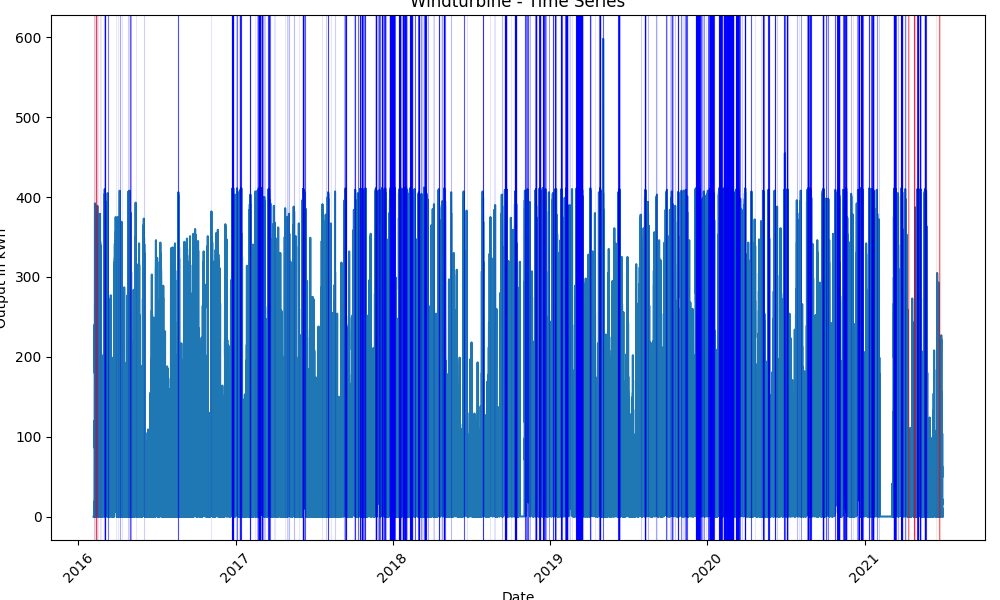
\includegraphics[width=\linewidth]{graphs/Windturbine - Time Series.png}
    \caption{Complete Power Output - Kelmarsh \#6}
    \label{fig:Kelmarsh-missing-values}
\end{figure}

Here it becomes visible that most of the missing values are all found in the beginning of the time series, this could be an indicator that not every wind mill was being monitored from the same time on wards as different magnitudes in the missing values for the different turbines show. As a result all missing values in the beginning are being dropped as well as all sequences in each time series with a duration of more than 3 hours since keeping these values does not hold any value for the forecasting task. These outages could be attributed to for example maintenance work. Sin

For the already mentioned problem of having too many outliers in 3 of 6 turbines remains. Outliers in this context have been defined as
\begin{equation}
    |\text{outlier}| >= 3 * \left( \frac{x - \mu}{\sigma} \right)
\end{equation}
the factor of three was chosen instead of the more usual two to account for extremes in wind speed especially in the coastal areas. To visualize the potential outliers all values for the Kelmarsh Wind park have been mapped as a kernel density estimation. The left figure \ref{fig:Kelmarsh-distribution} shows that the majority of values are centred around zero, hence no electricity output and presumably no wind speed. But there is also the practice of turning a turbine out of the wind if the situation demands it, hence no electricity production even though there would be enough wind. To test this hypothesis an deeper analysis of the turbine 6 was done to investigate how often this particular turbine was turned out of the wind. This was defined as 
\begin{equation}
    \text{out of wind} = \text{Wind speed (m/s)} > 3 \land \text{Power (kW)} < 1 
\end{equation}
resulting in $8705$ values being flagged, or equally $3.16 \%$ of all values. Therefor the data is being removed since the decision of turning a turbine out of the wind is influenced more by the stock exchange prices or the load factor of the electricity grid and has nothing to do with the prediction based on weather indicators. \par 
The extent can also be seen in the visualization of the $6^th$ turbine in the right figure \ref{fig:Kelmarsh-distribution}

\begin{figure}[h!]
    \centering
    \begin{subfigure}[b]{0.45\linewidth}
        \centering
        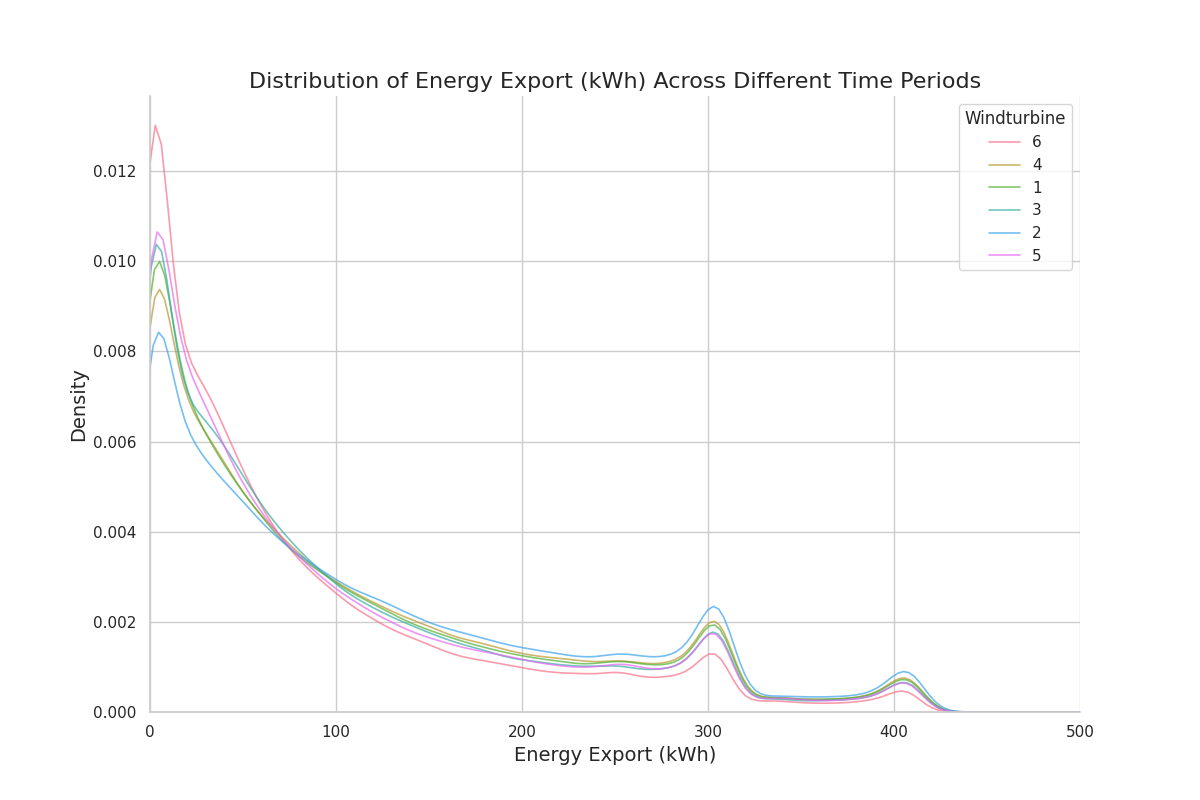
\includegraphics[width=\linewidth]{graphs/Kelmarsh_output_distribution.png}
        \caption{total}
    \end{subfigure}
    \begin{subfigure}[b]{0.45\linewidth}
        \centering
        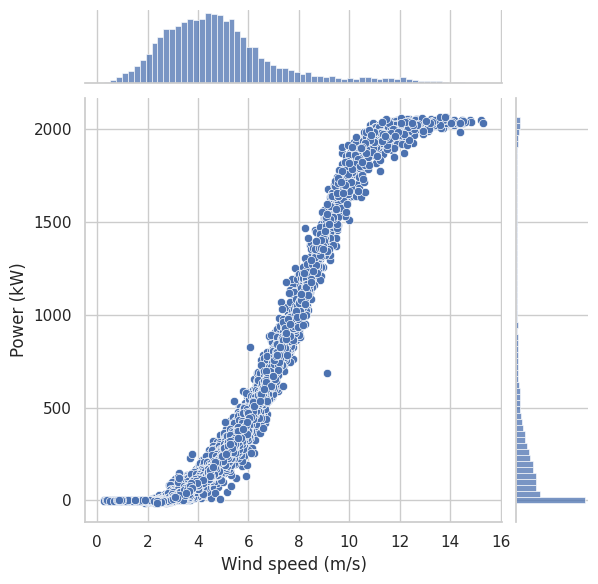
\includegraphics[width=\linewidth]{graphs/Corr_Wind_Power.png}
        \caption{\#6}
    \end{subfigure}
    \caption{Kelmarsh power distribution}
    \label{fig:Kelmarsh-distribution}
\end{figure}





\subsection{Industrial Electricity Consumption}






\section{Methodology}

The models selected for evaluation are several different transformer models, an LSTM model and a non-machine learning based model that serves as a benchmark for the other models. For the benchmark task, the Random Forest was chosen because of its numerous applications in the field of time series forecasting in previous work. The models that use deep neural networks are not written from scratch, but come from various publicly available libraries (PyTorch). These basic models are then fine-tuned using hyperparameter search. For the transformer models, various models from renowned papers as well as a self-made shallow transformer are selected to test whether the depth of the network has a large impact on the results. The forecast horizons are 1 hour, 24 hours and 96 hours, with the last forecast being the most difficult task. This last number was chosen because the weather forecasts are also produced for a 96-hour period. This rating is based on the total computational time to evaluate all models and the computational resources in terms of GPU/CPU and RAM usage.\par 

It is difficult to quantify whether a model provides a benefit in terms of increased predictive accuracy compared to the computational costs spent on development. Due to scalability, a small increase in accuracy can justify huge development costs when deployed at scale. The data is first pre-processed in a data pipeline to detect outliers and find missing values that could later affect the models. In a second step, the data is fed into the different models, and each of the datasets is compared against certain metrics to measure the performance of the models. Finally, the results are printed in tabular form and presented graphically for better comparability in the paper. \par 
Though an important question remains, how to assess the goodness of the models in a more qualitative way. Is accuracy more important, than training time and resources or is a intuitive interpretation for a broader audience also important?

The aim for the newly developed model is generalization with complex and less complex data, therefor it is not planned to include layers for extra steps found in other models such as seasonal decomposition or trend analysis.

\subsection{Model Evaluation}

To determine whether a Model is successful in their task, standardised methods of comparison are needed. These already exist for the accuracy, as the metric to determine the goodness of a model is measured in how small the error of a model is. These errors can be measured in different ways, with the most prominent ones in regression analysis being:

The Mean Absolute Error (MAE) is a widely used metric for evaluating the performance of regression models. It is defined as the average of the absolute differences between the predicted and actual values. Mathematically, it is expressed as:

\begin{equation}
\text{MAE} = \frac{1}{n} \sum_{i=1}^{n} \left| y_i - \hat{y}_i \right|
\end{equation}

where \(y_i\) and \(\hat{y}_i\) are the actual and predicted values, respectively, and \(n\) is the number of observations. MAE is easy to interpret and provides a linear penalty for each unit of difference between the predicted and actual values \cite{MAE_RMSE}.
Mean Absolute Percentage Error (MAPE) is another metric commonly used for evaluating regression models, particularly when the data spans several orders of magnitude. It is defined as:

\begin{equation}
\text{MAPE} = \frac{100}{n} \sum_{i=1}^{n} \left| \frac{y_i - \hat{y}_i}{y_i} \right|
\end{equation}

MAPE expresses the error as a percentage, making it unitless and easier to compare across different scales \cite{MAPE}.
Mean Squared Error (MSE) is a metric that measures the average of the squares of the errors between the predicted and actual values. It is defined as:

\begin{equation}
\text{MSE} = \frac{1}{n} \sum_{i=1}^{n} (y_i - \hat{y}_i)^2
\end{equation}

MSE penalizes larger errors more severely than smaller ones, making it sensitive to outliers \cite{MSE}.
Root Mean Squared Error (RMSE) is the square root of MSE and is defined as:

\begin{equation}
\text{RMSE} = \sqrt{\text{MSE}}
\end{equation}

RMSE has the same units as the dependent variable and is particularly useful when large errors are undesirable \cite{MAE_RMSE}.\par 

Utilizing each of these error metrics a wider range of potential problems and areas of interest (like the penalising of outliers) can be covered. But what is scarcely being looked upon are other metrics of evaluating models besides the accuracy, this includes resource efficiency and computational requirements linked to that the time to train and an intuitive interpretation of the results. In this thesis, these measurements are playing a bigger role in evaluating models besides the accuracy. Especially resource efficiency is playing a bigger role as shown by \cite{AI_energy_consumption} and \cite{resource_awareness}. One of the problems lies in size and complexity of machine learning models which alongside the volume of data required for the training have been experiencing exponential growth, thereby demanding more computational resources. This trend has outpaced the advancements in computing hardware platforms, storage infrastructure, and networking capabilities, leading to sustainability challenges. Some papers such as \cite{Informer} have implemented some aspects to reduce the computational efficiency, but their idea was more about training time than resource efficiency. \par 
The problem with evaluating the resource efficiency, is the lack of a proper framework and standardised measurements. It is not in the scope if this thesis to develop such frameworks, but to map the resources used to train different models on the same data and further the time spend during the whole development process on training, testing and performing inference on cloud computers is mapped, evaluated and critically viewed for improvements and saving opportunities.


\subsection{Linear Models}

The linear model used in this thesis is nothing new, but is regarded as a benchmark towards the other models. To compare the more complex models to a very simple model, with the expectation that the more complex models outperform the simpler models. If that is not going to be the case or they achieve similar results, than the models are regarded as failures and are being discarded. \par 

The linear model is based on the same starting conditions as the other models, the same lags, the same variables in a multivariate context and the same data for the train, validation and test sections. What is not being included is a layer for seasonal decomposition as well as trend cycles, since the aim is to develop models can perform reasonable well without these to increase their generalization performance. 

\subsection{Machine Learning Models}


\subsection{DeepLearning Models}

The goal in this section is to create a distinct Transformer model for time series forecasting, not from scratch but to dissect several different published models and evaluate what each of these models did differently and if the innovative parts is beneficial to this context and data. To get an understanding of the models one has to first in what regard each one differentiates from the vanilla model and also why and how they did it. \par 
Since the DeepLearning Models are in the centre of the research a thorough valuation of the performance of these models is conducted. With the different architectures different strategies to solve the same problem are being introduced. Therefor the results of all transformer models are compared separately in more depth, to investigate which of the architectures and strategies achieve the best performance. 

\subsubsection{Vanilla Transformer}

The vanilla transformer represents a version that is close to the original model presented by \cite{vanilla-transformer} that utilises the attention mechanism and is not optimised in any way to a time series forecasting role, hence it has no additional layers to perform seasonal decomposition or other methods.

\subsubsection{Informer}

The Informer is a model developed by \cite{Informer} that sets itself apart by enabling multivariate instead of univariate probabilistic time series forecasting. The most distinct noticeable changes are the reduction of the computational requirements to calculate the attention mechanism and reduces the memory usage of the encoder/decoder layers. The first improvement refers to the complexity of calculation for the self-attention in the vanilla model, this can be described with the formula
\begin{equation*}
    O(T^2 \cdot D)
\end{equation*}
where $T$ is the length of the time series and $D$ is the dimension of the hidden states. The problem here lies in $T^2$ which explodes in the case of long sequences. Therefore the authors have proposed a different method called \textit{ProbSparse} that calculates the complexity of the self-attention calculation as
\begin{equation*}
    O(T \cdot log{T}) .
\end{equation*}
The idea is the differentiation between 'active' and 'lazy' parts where respective dot products contribute in different magnitudes towards the attention mechanism. The 'lazy' parts with a negligible contribution are left out and only the 'active' parts are considered



    Quadratic computation of canonical self-attention:
    The vanilla Transformer has a computational complexity of  where TT is the time series length and DD is the dimension of the hidden states. For long sequence time-series forecasting (also known as the LSTF problem), this might be really computationally expensive. To solve this problem, Informer employs a new self-attention mechanism called ProbSparse attention, which has time and space complexity.
    
    Memory bottleneck when stacking layers:
    When stacking NN encoder/decoder layers, the vanilla Transformer has a memory usage of , which limits the model's capacity for long sequences. Informer uses a Distilling operation, for reducing the input size between layers into its half slice. By doing so, it reduces the whole memory usage to be.

Another interesting aspect that this paper utilises is the use of \textit{Probabilistic Time Embedding}. This method does not only encodes the data to vectors, but does also take into account the uncertainties associated with the given time information. This is particularly useful in contexts where the time variable plays a crucial role and its varying effect can not be mapped in a deterministic way. The idea behind this is that an embedding for a particular time step is not fixed but can be a distribution. Therefore, multiple possible embeddings could represent a single time step, capturing the inherent uncertainty or variability at that time. Hence a distribution in this context shows a set of possible vectors that could represent the embedding of a particular time series, instead of being listed as a single vector. Each vector sampled from this distribution would be a valid representation of the time series, allowing the model to capture the uncertainty associated with it. The reason why this can be useful in the context of Time Series Forecasting is due to the fact that the state of the system could be uncertain or subject to external factors not included in the model. In this cas, using a distribution over embeddings can help the model account for the corresponding uncertainty during training and inference.

\subsubsection{Autoformer}

\cite{autoformer}




\newpage

\printbibliography

\end{document}